\documentclass[12pt,a4paper]{article}

\usepackage{ctex}   				% 提供中文支持,包括中文文档的字体、字号、标点、章节标题等
\usepackage[colorlinks=false]{hyperref}		% 处理超链接,包括文档内的交叉引用和文献引用,以及生成PDF文档时的超链接,可选参数关闭了超链接的颜色
\usepackage{times}					% 设置文档使用Times字体
\usepackage{amsmath}				% 提供了许多数学排版的增强功能包含了丰富的数学环境、数学命令和数学符号以及众多用于排版数学公式的命令
\usepackage{amsfonts}				% 提供了额外的数学字体如黑板粗体、花体字母
\usepackage{amssymb}				% 包含了许多额外的数学符号,如各种箭头、集合运算符、关系符号等
\usepackage{mathrsfs}				% 提供了一种额外的花体字母
\usepackage{graphicx}				% 用于插入和处理图形
\usepackage{subcaption}				% 允许在一个浮动体中包含多个子图
\usepackage{float}					% 提供浮动体的控制
\usepackage{adjustbox}				% 提供图形和表格的调整选项
\usepackage{bibentry}				% 提供\bibentry{key}命令,可以在文档中嵌入引用文献的完整内容,允许在文档正文中显示完整的文献条目,而不是仅在参考文献列表中显示
\usepackage[numbers]{natbib}		% 提供了更强大和灵活的文献引用功能,支持多种引用风格
\usepackage{abstract}				% 用于定制摘要的格式
\usepackage{xcolor}					% 提供颜色相关的命令和选项
\usepackage{url}					% 提供了处理超链接和网址的命令,支持在文档中插入可点击的链接
\usepackage{bm}						% 允许在数学模式中使用\bm命令给符号加粗
\usepackage{multirow}				% 用于在表格中合并多行
\usepackage{booktabs}				% 用于改进表格的横线显示,提供了更美观的水平线风格
\usepackage{epstopdf}				% epstopdf 将 EPS 转换为PDF格式
\usepackage{epsfig}					% epsfig 提供了在文档中插入EPS图形的命令。
\usepackage{longtable}				% 提供了 longtable 环境,该环境允许表格在页面之间分页,保证表头和表尾在每一页都能正确显示
\usepackage{supertabular}			% 提供了 supertabular 环境,类似于 longtable,允许表格在页面之间分页,但 supertabular 具有更多的自定义选项
\usepackage{algorithm}				% 提供了 algorithm 环境,用于排版算法。允许用户在文档中创建算法块,并提供了一些用于控制算法格式和样式的选项。
\usepackage{algorithmic}			% 提供了一系列用于排版伪代码的命令,允许用户使用伪代码描述算法的执行步骤,提供了类似于if, while, for等关键字的命令。
\usepackage{changepage}				% 允许用户使用伪代码描述算法的执行步骤,提供了类似于 if, while, for 等关键字的命令。
\usepackage{enumerate}				% 允许用户自定义列表项的标签和格式
\usepackage{indentfirst}			% 让每个章节的第一个段落首行缩进,符合中文排版习惯
\usepackage[left=2.50cm,right=2.50cm,top=2.80cm,bottom=2.50cm]{geometry}	% 提供了设置文档页边距、纸张大小等的命令
\usepackage{fancyhdr}				% 允许用户自定义页眉和页脚的内容、样式和位置
\usepackage{caption}				% 提供了更多的选项,允许用户自定义图表标题的字体、大小、对齐方式等
\usepackage{lipsum}					% 自动生成虚拟文本
\usepackage{multicol}				% 允许在文档中创建多列布局
\usepackage{lettrine}				% 用于创建大型首字母(drop cap)
\usepackage{esint}					% 提供了更多的积分符号
\usepackage{tikz}					% 用于创建图形和绘制矢量图
\usepackage{caption}				% 允许用户设置图表标题的格式和样式
\usetikzlibrary{arrows.meta}        % 为 tikz 宏包提供更多箭头样式
\usepackage{pgfplots}				% 基于TikZ,专门用于绘制二维和三维的数据图
\usepackage{tikz-3dplot}			% 用于在TikZ中简化三维坐标系的创建和绘制
\usepackage{setspace}				% 用来调整行间距
\usepackage{yhmath}					% 主要提高了一些数学符号的显示,比如扩展的括号和根号等
\usepackage{gensymb}				% 供了一套用于科学和工程文档的通用符号命令
\usepackage{upgreek}				% 提供 \upmu 等正体希腊字母
\usepackage{textcomp}				% 提供了 \textmu 等正文中使用希腊字母

%%%%%%%%%%%%%%%%%%%%%%%%%%%%%%%%%%%%%%%%%%%%%%%%%%%%%%%%

% 这些宏包提供了很多符号,但是会改变字体,这些字体不是最广泛接受的,不建议使用
%\usepackage{newtxmath}				% 提供与Times Roman文本字体相配套的数学字体和符号。它是txfonts宏包的后续和改进版本
%\usepackage{newtxtext}				% 同上,文字部分
%\usepackage{txfonts}				% 提供平行符号等的包,修改数学字体,对应于Times Roman字体样式,但是似乎会和其他包冲突
%\usepackage{pxfonts}				% 提供平行符号等的包,修改数学字体,使用Palatino风格字体,但是似乎会和其他包冲突,


\pagestyle{fancy}
\hypersetup{colorlinks=false,linkbordercolor=white,allcolors=white,citebordercolor=white,runcolor=white,allcolors=white,filecolor=white,linkcolor=white}
\captionsetup[figure]{name=\fontsize{10pt}{15pt}\selectfont Figure} 
\captionsetup[table]{name=\fontsize{10pt}{15pt}\selectfont Table} 

%%%%%%%%%%%%%%%%%%%%%%%%%%%%%%%%%%%%%%%%%%%%%%%%%%%%%%%%

\renewcommand{\abstracttextfont}{\fangsong} 
\renewcommand{\abstractname}{\textbf{摘\quad 要}} 
\renewcommand{\baselinestretch}{1.5}
\renewcommand\parallel{\mathrel{/\mskip-2.5mu/}} % 定义斜的平行符号

\newcommand{\red}[1]{\textcolor[rgb]{1.00,0.00,0.00}{#1}}
\newcommand{\blue}[1]{\textcolor[rgb]{0.00,0.00,1.00}{#1}}
\newcommand{\green}[1]{\textcolor[rgb]{0.00,1.00,0.00}{#1}}
\newcommand{\darkblue}[1]{\textcolor[rgb]{0.00,0.00,0.50}{#1}}
\newcommand{\darkgreen}[1]{\textcolor[rgb]{0.00,0.37,0.00}{#1}}
\newcommand{\darkred}[1]{\textcolor[rgb]{0.60,0.00,0.00}{#1}}
\newcommand{\brown}[1]{\textcolor[rgb]{0.50,0.30,0.00}{#1}}
\newcommand{\purple}[1]{\textcolor[rgb]{0.50,0.00,0.50}{#1}}

%%%%%%%%%%%%%%%%%%%%%%%%%%%%%%%%%%%%%%%%%%%%%%%%%%%%%%%%

\setlength{\parindent}{0pt}			% 取消自动段首缩进

%%%%%%%%%%%%%%%%%%%%%%%%%%%%%%%%%%%%%%%%%%%%%%%%%%%%%%%%
% 自定义巨型算符

\makeatletter
\DeclareRobustCommand\bigop[1]{%
	\mathop{\vphantom{\sum}\mathpalette\bigop@{#1}}\slimits@
}
\newcommand{\bigop@}[2]{%
	\vcenter{%
		\sbox\z@{$#1\sum$}%
		\hbox{\resizebox{\ifx#1\displaystyle.9\fi\dimexpr\ht\z@+\dp\z@}{!}{$\m@th#2$}}%
	}%
}
\makeatother

\newcommand{\bigK}{\DOTSB\bigop{\mathrm{K}}}

%%%%%%%%%%%%%%%%%%%%%%%%%%%%%%%%%%%%%%%%%%%%%%%%%%%%%%%
% 封面信息

\title{\fontsize{18pt}{27pt}\selectfont{\heiti 第八章作业: 振动}} 
\author{\fontsize{12pt}{18pt}\selectfont {\fangsong  林海轩}\\\fontsize{10.5pt}{15.75pt}\selectfont{\fangsong(复旦大学 物理学系)}} 
\date{}

%%%%%%%%%%%%%%%%%%%%%%%%%%%%%%%%%%%%%%%%%%%%%%%%%%%%%%%%
% 注意这部分代码将全角的逗号句号转换为了半角的逗号句号且半角逗号后面跟了一个空格,要求用xelatex编译,但模板撰写的时候默认用pdflatex,不推荐使用

%\catcode`,=\active
%\newcommand{,}{, }

%\catcode`。=\active
%\newcommand{。}{.}

%\catcode`:=\active
%\newcommand{:}{: }
%%%%%%%%%%%%%%%%%%%%%%%%%%%%%%%%%%%%%%%%%%%%%%%%%%%%%%%%
% 自己编写的命令,用于生成不编号但计入目录的标题

\newcommand{\nonumbersection}[1]{
	\section*{#1}
	\addcontentsline{toc}{section}{#1}
}
\newcommand{\nonumbersubsection}[1]{
	\subsection*{#1}
	\addcontentsline{toc}{subsection}{#1}
}
%%%%%%%%%%%%%%%%%%%%%%%%%%%%%%%%%%%%%%%%%%%%%%%%%%%%%%%%
 
\begin{document}
	
	\lhead{} 
	\chead{} 
	\rhead{} 
	\lfoot{}
	\cfoot{\thepage} 
	\rfoot{} 
	
	\maketitle
	
	\begin{abstract}
		\fangsong 为了以后能摆大烂而创造了一个模板,为了展现转行效果而开始啊对对对对对对对对对对对对对对对
	\end{abstract}
	
	\begin{adjustwidth}{1.06cm}{1.06cm}
		\fontsize{10.5pt}{15.75pt}\selectfont{\heiti{关键词:}\fangsong{摆大烂、啊对对对}}\\
	\end{adjustwidth}
	
	\begin{center}% 居中处理
	{\textbf{Abstract}}% 英文摘要
	\end{center}
	\begin{adjustwidth}{1.06cm}{1.06cm}% 英文摘要内容
		\hspace{1.5em}In order to improve my computer and English skills, please allow me to complete this physics homework in English context with \LaTeX, so as to improve my professional level. Sorry for the inconvenience!
	\end{adjustwidth}
	
	\newpage
	
	\renewcommand{\contentsname}{Contents}
	\tableofcontents
	
	\newpage
	
	\section{Fucking Blind Passenge}
	\subsection{Fuck here}
	\subsubsection{Yes Just Fuck}
	\lettrine{T}{his} is an Fucking article i write to practice my \LaTeX\ level u Know uh?	"In the ever-evolving landscape of modernity, the paradigm shift towards innovative methodologies has become a cornerstone of progressive discourse. $\upmu$\textmu
	\begin{equation}
		\cfrac{a_1}{b_1+\cfrac{a_2}{b_2+\cfrac{a_3}{b_3+\cdots}}}=\bigK_{N=1}^\infty\frac{a_N}{b_N}
	\end{equation}
	As we navigate the complexities of our interconnected world, it is incumbent upon us to leverage synergies and catalyze holistic solutions. $\bigK\limits_{N=1}^\infty a_N/b_N$ The dynamic interplay between technological advancements and socio-cultural dynamics propels us into an era of unprecedented possibilities.
	
	\lipsum[1-2]
	\subsubsection{OHHHHHH! HOW GREAT!}
	\begin{multicols}{2}
	\lipsum[66-70]
	\end{multicols}
	\subsection{Sh*t Making Love}
	\subsubsection{Yeap Fuck me}
	\lipsum[6-7]\footnote{The Whole Paragraph is deliver by Lipsum.}
	\subsection{Make love with ur mum}
	\subsubsection{There are too much dirty words}
	\lipsum[1-4]
	\subsubsection{Mark Zhong I want to Fuck U}
	\lipsum[2-3]
		\begin{figure}[H]
		\begin{minipage}{0.45\textwidth}
			\centering
			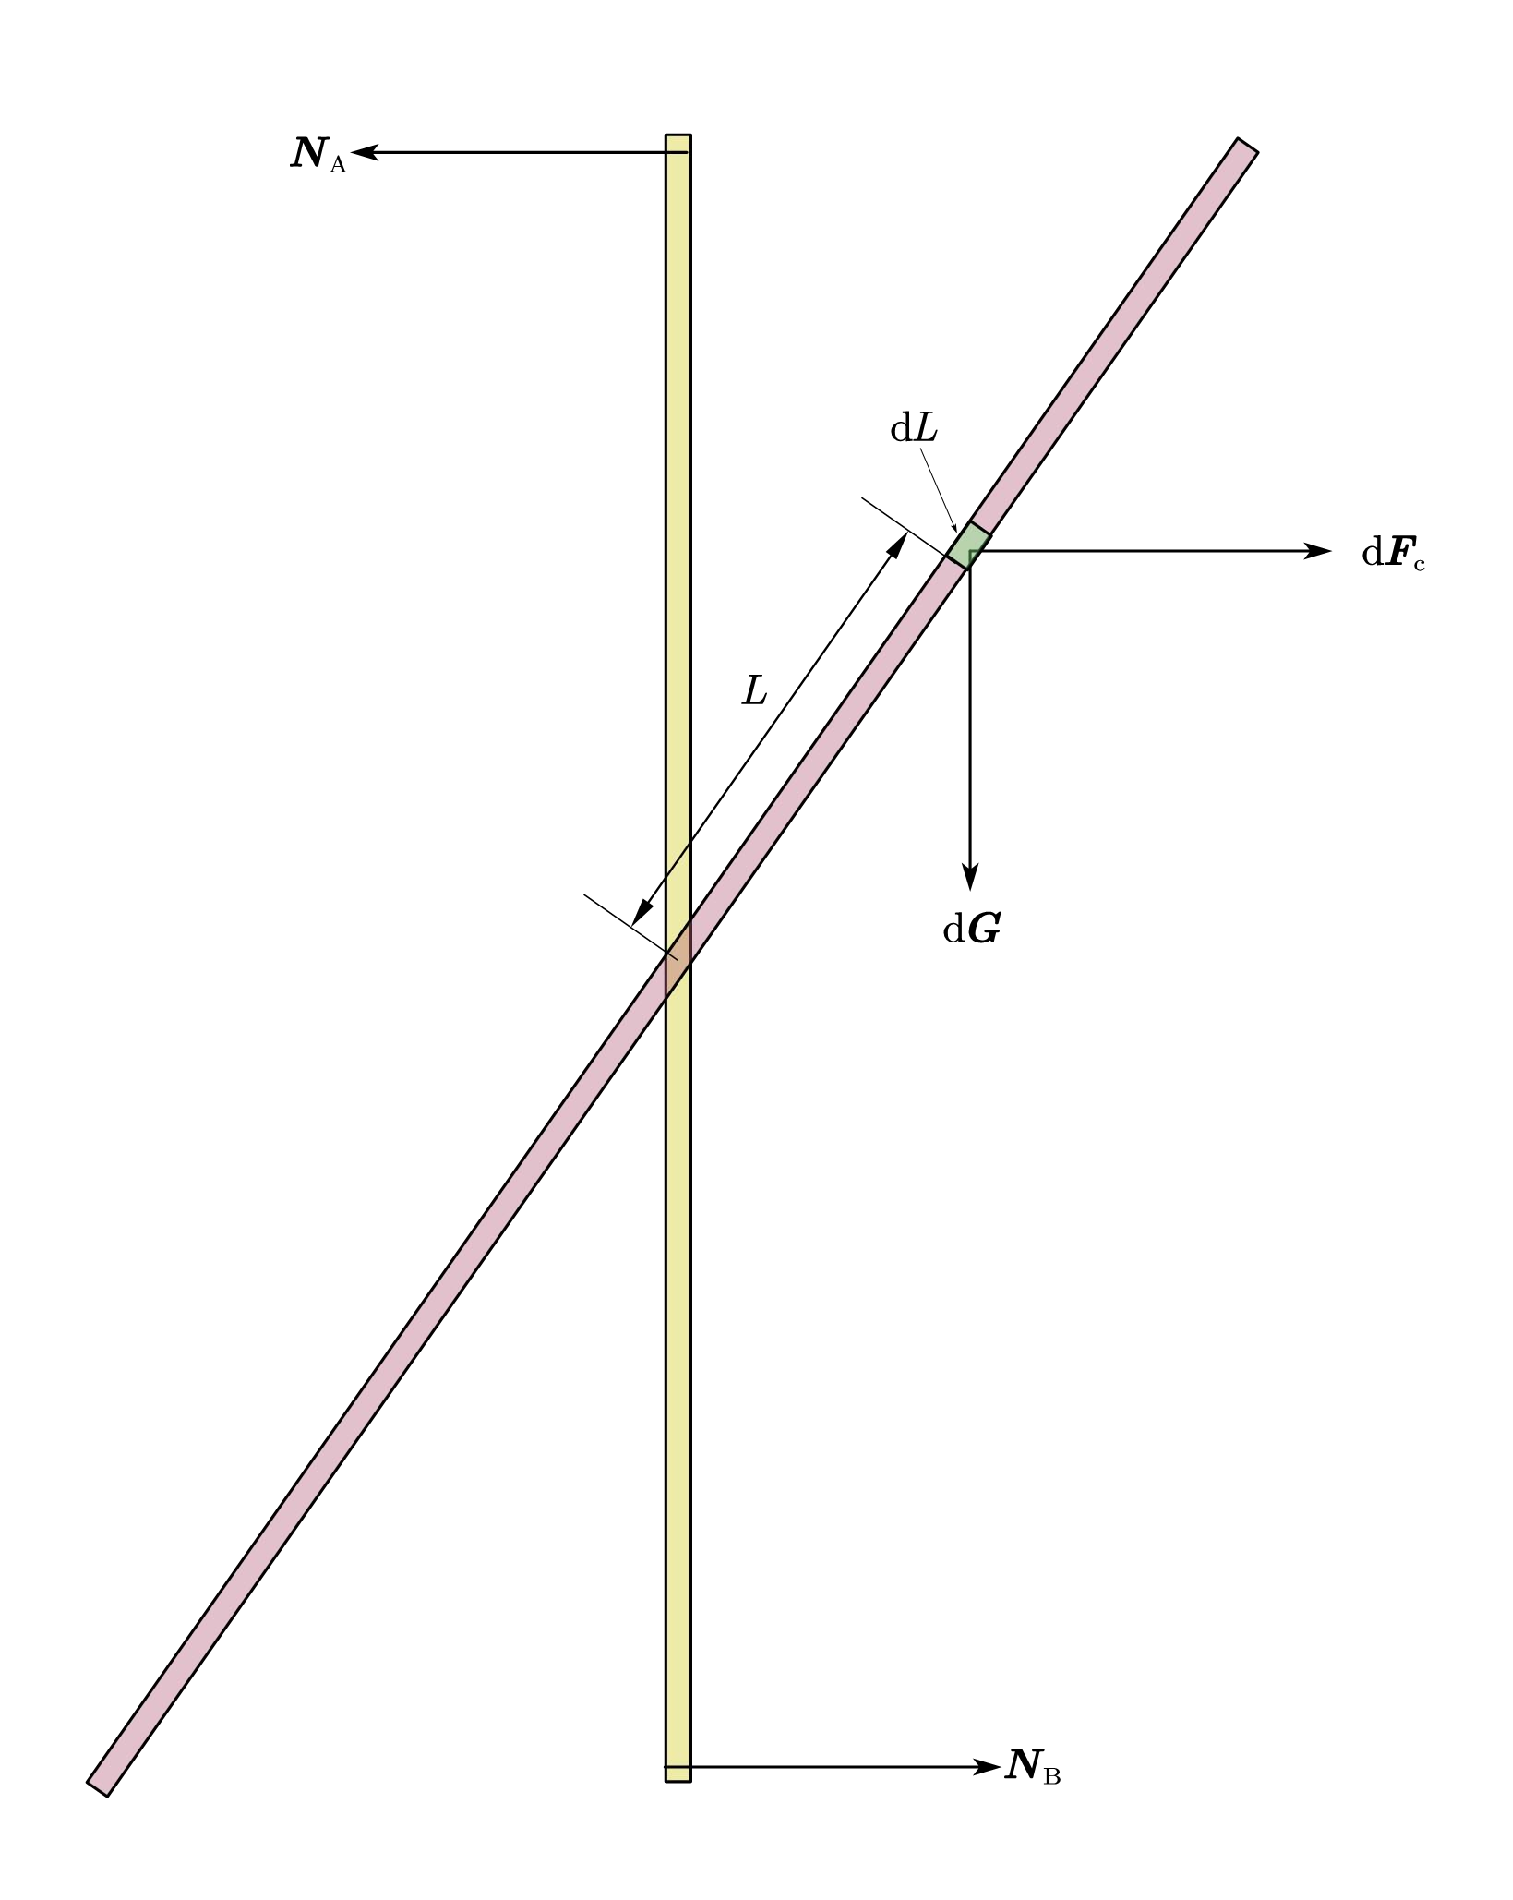
\includegraphics[width=\linewidth]{C:/Users/Administrator/Desktop/VScode/LaTeX/EarlyPic/6-12}
			\caption*{}
		\end{minipage}
		\hfill
		\begin{minipage}{0.45\textwidth}
			\centering
			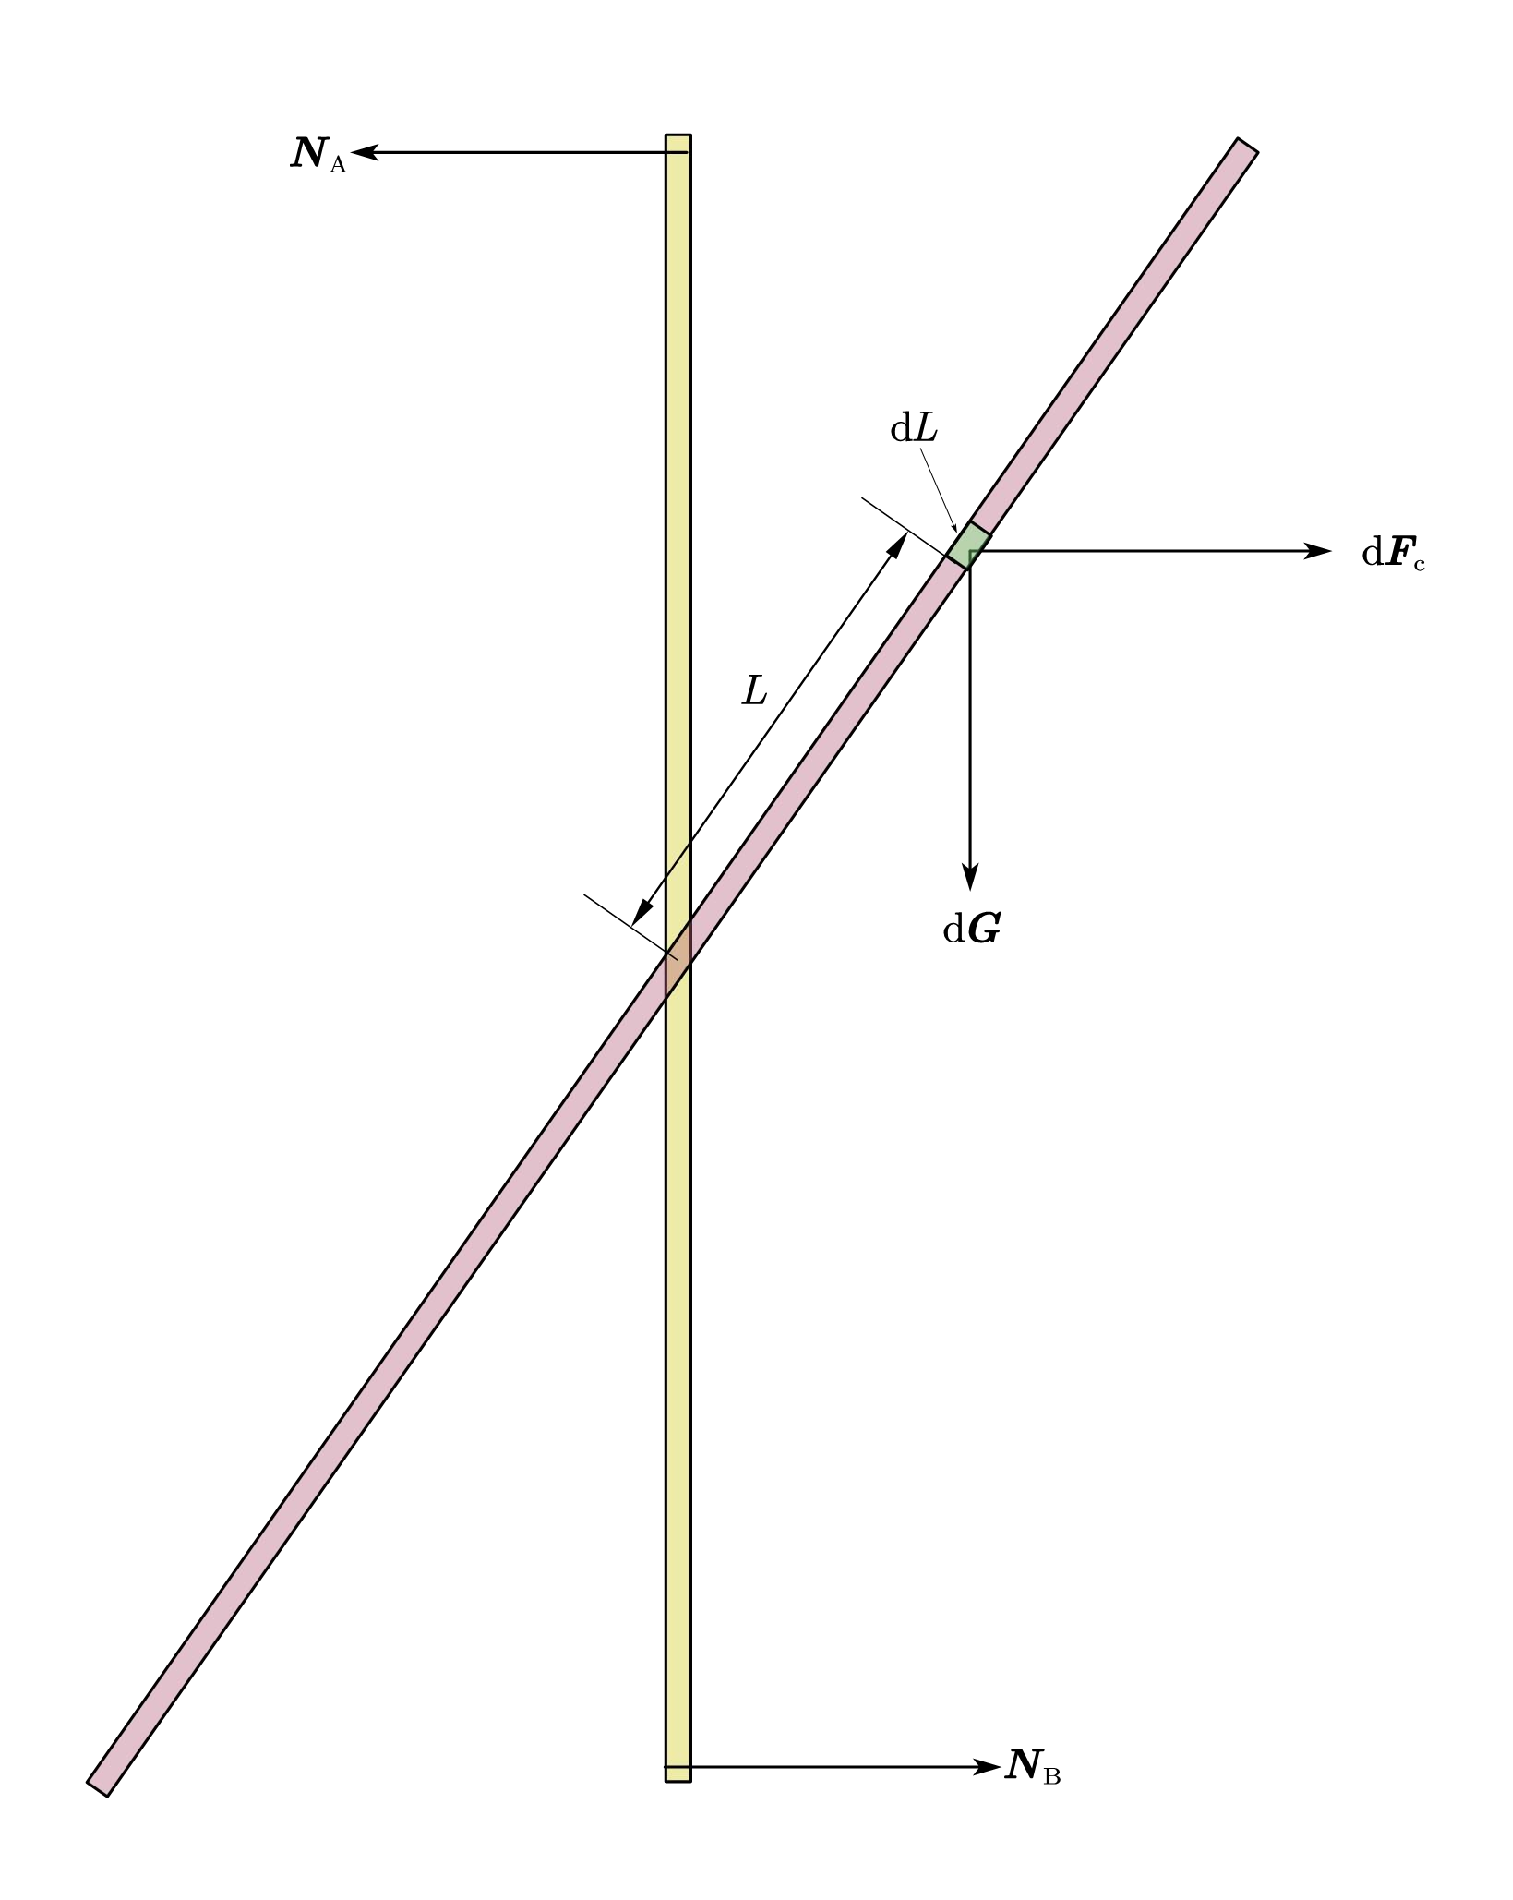
\includegraphics[width=\linewidth]{C:/Users/Administrator/Desktop/VScode/LaTeX/EarlyPic/6-12}
			\caption*{}
		\end{minipage}
		\end{figure}
		用这个方法可以放多个图片.
	\subsubsection{Welcome to Fuck Yxx}
	\lipsum[99]
			
	\section{Bully Guy}
	\subsection{Nirge fuck}
	\subsubsection{Take it Ease}
	\lipsum[1-2]
	\begin{equation}
		\varPhi_E=\varoiint_S\boldsymbol{E}\cdot\mathrm{d}\boldsymbol{S}
	\end{equation}
	\subsubsection{I Love u Babe}
	\lipsum[3-5]
	\subsection{KLKL}
	\subsubsection{TOO abab}
	\lipsum[6-7]\footnote{The Whole Paragraph is deliver by Lipsum.}
	\subsection{ZLblblbl}
	\subsubsection{Thats OK babe}
	\lipsum[1-4]
	\subsubsection{I promise}
	\lipsum[2-3]
	\subsubsection{Just GOO}
	\lettrine{F}{uuuuuuuuuuking} In conclusion, the tapestry of progress is woven with the threads of innovation, collaboration, and enviro$\mathscr{L}$nmental stewardship. As we stand at the crossroads of limitless possibilities, it is our collective responsibility to embark on a journey towards a more enlightened and sustainable future."
	\lipsum[99]
	
	\section{中文测试语段}
	\subsection{不必理会太多}
	\begin{multicols}{2}
		在这个充满奇迹和可能性的时代,我们置身于科技与人文交融的璀璨星空之下。如同一幅幅抽象的艺术画作,我们的生活也变得丰富多彩,每一刻都充满了未知的惊喜和挑战。			
		
		\lipsum[1-3]
		
		随着全球化的推动,我们发现自己越来越成为这个地球村中的一员。文化的碰撞和融合使得我们拥有了更广阔的视野,也让我们深感世界的多姿多彩。正是在这个多元文化的交汇中,我们的心灵得以不断升华,成为更为包容和理解的个体。
		
		而在信息时代的冲击下,我们的生活变得更加数字化和虚拟化。互联网的发展让我们仿佛置身于一个全球大脑中,信息传递的速度之快让人目不暇接。在这个信息的海洋中,我们需要学会筛选和理解,培养批判性思维,以更加明智的方式面对激流涌进的信息浪潮。
	
		与此同时,环境问题也成为我们不能忽视的焦点。气候变化、生态平衡的破裂,这些问题影响着我们的生存和发展。在这个关键时刻,我们需要共同努力,探索可持续的发展之路,保护我们共同的家园。
		
		在职场中,竞争日益激烈,我们需要不断提升自己的职业素养。创新和创业精神成为了前行的动力,我们要敢于突破传统,勇攀高峰。与此同时,团队协作也变得愈发重要,因为每一个个体都是整个团队中不可或缺的一环。
		
		总的来说,在这个充满变革和机遇的时代,我们需要拥抱变化,保持对未来的好奇心,勇敢地追逐梦想。让我们携手前行,共同书写属于我们的时代史诗,创造更加美好的明天。
	\end{multicols}
	\subsubsection{全都是我瞎几把写的}
		"在现代不断演变的格局中,朝着创新方法的范式转变已成为进步讨论的基石。在我们航行于互联世界的复杂性中,我们有责任充分利用协同效应,催生全面的解决方案。技术进步与社会文化动态之间的动态互动推动我们进入前所未有的可能性时代。
		
		在前沿研究与发展领域,跨学科方法的综合开创了新的领域。人工智能和人类创造力的并置为变革性突破打开了新的途径。人与机器之间的这种共生关系为未来铺平了道路,在那里现实与虚拟之间的界限无缝融合。
		
		指数的显示似乎是有点问题的,以下运用 frac 指令:
		$$
		k = A\mathrm{e}^{-\frac{E_a}{k_\mathrm{B}T}}
		$$
		
		以下运用 dfrac 指令:
	 	$$
		k = A\mathrm{e}^{-\dfrac{E_a}{k_\mathrm{B}T}}
		$$
		
		以下运用 tfrac 指令:
		$$
		k = A\mathrm{e}^{-\tfrac{E_a}{k_\mathrm{B}T}}
		$$
		
		gtp建议
		
		\[ k = A e^{-\frac{\scriptstyle E_a}{\scriptstyle k_B T}} \]
		
		
		或者细调间距
		
		\[ k = A e^{-\frac{\scriptstyle E_a}{\scriptstyle\, k_B T}} \]
		
		此外,在我们寻求可持续解决方案的过程中,环境意识的时代已经上演。采用环保实践的必要性在董事会和学术机构中回响。利用可再生能源并拥抱循环经济原则是迈向更绿色未来的关键步骤。
		
		总之,进步的画卷是由创新、合作和环境管理的纱线编织而成的。当我们站在无限可能的十字路口时,我们有责任共同踏上通向更加开明和可持续未来的旅程。"
	\subsubsection{变成光守护麻衣学姐}
	医生的建议:
	医生对患者说:“您的血型是B,但不用担心,这只是表示您缺少点阳光,多晒晒太阳就好了。”
	
	职业选择:
	一位朋友对另一位说:“我决定当心理医生了。”
	朋友问:“为什么?”
	他回答:“我觉得我有很多问题,而且我喜欢对别人指手画脚。”
	
	失业的鸡:
	为什么鸡失业了?
	因为它被辞退了,老板说它的表现在蛋上。
	
	寿命的秘密:
	有人问寿命的秘密是什么?
	
	此处 yhmath 宏包修改了根号使得其有更好的显示
	$$
	\sqrt{\sqrt{\sqrt{\sqrt{\sqrt{\sqrt{\sqrt{\sqrt{\sqrt{\sqrt{\sqrt{\sqrt{\sqrt{\sqrt{\sqrt{\sqrt{\sqrt{\sqrt{\sqrt{x}}}}}}}}}}}}}}}}}}}
	$$
	
	
	%$$
	%C_1\varparallel C_2
	%$$
	其实,就是不要去医院,那里的发现率太高了。
	
	拒绝的理由:
	一个程序员向女友求婚,她说:“不,我喜欢你,但你总是在循环。”
	
	不高兴的鱼:
	为什么鱼总是那么不高兴?
	因为它们总是在水里,但永远也不能上岸看看世界。
	
	怪诞的愿望:
	有一天,一个人遇到了一个神仙,被赋予了三个愿望。他说:“首先,我想拥有无限的财富。”
	神仙说:“好的,你的第一个愿望已经实现了。”
	他接着说:“其次,我想拥有永远的青春。”
	神仙说:“好的,你的第二个愿望也实现了。”
	他微微一笑:“最后,我想有点小毛病,你懂的,让我显得普通一点。”\textsuperscript{\cite{QLN2021}}
	神仙若有所思地点了点头:“好吧,你的第三个愿望也实现了,你现在是个程序员了。”\cite{PCD}
	\section{数学物理画图测试语段}
	\lettrine{S}{o} here is going to 测试\textbf{数学物理方程}的写作。在LaTeX中,runcolor通常不是一个通用的术语或宏包。可能是一种自定义命令、宏包或者文档类的名称。如果你能提供更多上下文或者详细信息,我将更容易提供帮助。如果你指的是特定的宏包、文档类或者自定义命令,请提供更多的细节,以便我更好地理解你的问题。
	\subsection{Let Try it!}
	\begin{tabular}{|c|c|c|c|c|}
		\hline
		语文 & 数学 & 英语 & 物理 & 化学 \\
		\hline 
		121 & 149 & 141 & 95 & 92 \\
		\hline
	\end{tabular}
	\begin{table}[H]
		\centering
			\begin{tabular}{|c|c|c|c|c|}
			\hline
			语文 & 数学 & 英语 & 物理 & 化学 \\
			\hline 
			121 & 149 & 141 & 95 & 92 \\
			\hline
			\end{tabular}
	\end{table}
	\vspace{-12pt}
	\lipsum[1-2]
	
	\subsubsection{tikz宏包的使用}
	第一点,绘制直线和矩形。
	
	\begin{figure}[htp]
		\centering
		\begin{tikzpicture}
			\draw (0,0)--(2,2); 
		\end{tikzpicture}
		\caption{直线}
	\end{figure}
	
	这就是基本格式,放在浮动体环境,这样才可以灵活设置形式,位置参数[htp]表示首选将图形放在代码所在的位置,如果不行则放在页面的顶部,如果还不行则放在一个包含浮动体的页面,$\backslash$centering 表示浮动体设置在中间,再开始tikz的环境,最后 $\backslash$caption\{\} 用来命名。
	
	draw是有可选参数的。

	\begin{figure}[htbp]
		\centering
		\subfloat{
			\begin{tikzpicture}
				\draw[->] (0,0)--(2,2); 
			\end{tikzpicture}}
			\caption{画箭头}
		\subfloat{
			\begin{tikzpicture}
				\draw[<->] (0,0)--(2,2); 
			\end{tikzpicture}}
			\caption{画双向箭头}
	\end{figure}

	\begin{figure}[htp]
		\centering
		\begin{tikzpicture}
			\draw[|<->|] (0,0)--(2,2); 
		\end{tikzpicture}
		\caption{画带横线的箭头}
	\end{figure}
	
	当然还可以设置箭头的样式。
	
	\begin{figure}[H]
		\centering
		\begin{tikzpicture}[>=latex]
			\draw[->] (0,0)--(2,2); 
		\end{tikzpicture}
		\caption{}
	\end{figure}
	
	\begin{figure}[H]
		\centering
		\begin{tikzpicture}[>=stealth]
			\draw[->] (0,0)--(2,2); 
		\end{tikzpicture}
		\caption{}
	\end{figure}
	
	也可以画不同样式的线.
	
	\begin{figure}[H]
		\centering
		\begin{tikzpicture}
			\draw[dashed] (0,0)--(5,0);
		\end{tikzpicture}
		\caption{}
	\end{figure}
	\begin{minipage}{0.5\textwidth}
		\centering
		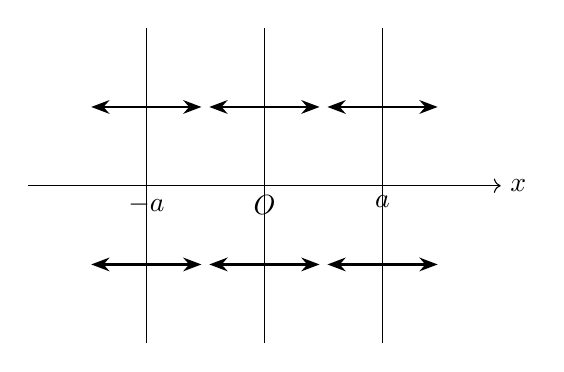
\begin{tikzpicture}
			\draw[->] (-3, 0) -- (-1.5, 0) node[below] {$-a$} -- (0, 0) node[below] {$O$} -- (1.5, 0) node[below] {$a$} -- (3, 0) node[right] {$x$};
			\draw (-1.5, -2) -- (-1.5, 2) (0, -2) -- (0, 2) (1.5, -2) -- (1.5, 2);
			\draw[-Stealth, thick] (-1.5, 1) -- (-0.8, 1);
			\draw[-Stealth, thick] (-1.5, 1) -- (-2.2, 1);
			\draw[-Stealth, thick] (-1.5, -1) -- (-0.8, -1);
			\draw[-Stealth, thick] (-1.5, -1) -- (-2.2, -1);
			\draw[-Stealth, thick] (0, 1) -- (-0.7, 1);
			\draw[-Stealth, thick] (0, 1) -- (0.7, 1);
			\draw[-Stealth, thick] (0, -1) -- (-0.7, -1);
			\draw[-Stealth, thick] (0, -1) -- (0.7, -1);
			\draw[-Stealth, thick] (1.5, 1) -- (0.8, 1);
			\draw[-Stealth, thick] (1.5, 1) -- (2.2, 1);
			\draw[-Stealth, thick] (1.5, -1) -- (0.8, -1);
			\draw[-Stealth, thick] (1.5, -1) -- (2.2, -1);
		\end{tikzpicture}
		\captionof*{figure}{Befor each electric field is superimposed} % 需要 caption 宏包
		% 或者如果不想用 caption 宏包:
		%\textbf{BE}
	\end{minipage}
	\begin{minipage}{0.5\textwidth}
		\centering
		\begin{tikzpicture}
			\draw[->] (-3, 0) -- (-1.5, 0) node[below] {$-a$} -- (0, 0) node[below] {$O$} -- (1.5, 0) node[below] {$a$} -- (3, 0) node[right] {$x$};
			\draw (-1.5, -2) -- (-1.5, 2) (0, -2) -- (0, 2) (1.5, -2) -- (1.5, 2);
			%\draw[-Stealth, thick] (-1.5, 1) -- (-0.8, 1);
			\draw[-Stealth, thick] (-1.5, 1) -- (-2.2, 1);
			%\draw[-Stealth, thick] (-1.5, -1) -- (-0.8, -1);
			\draw[-Stealth, thick] (-1.5, -1) -- (-2.2, -1);
			%\draw[-Stealth, thick] (0, 1) -- (-0.7, 1);
			%\draw[-Stealth, thick] (0, 1) -- (0.7, 1);
			%\draw[-Stealth, thick] (0, -1) -- (-0.7, -1);
			%\draw[-Stealth, thick] (0, -1) -- (0.7, -1);
			%\draw[-Stealth, thick] (1.5, 1) -- (0.8, 1);
			\draw[-Stealth, thick] (1.5, 1) -- (2.2, 1);
			%\draw[-Stealth, thick] (1.5, -1) -- (0.8, -1);
			\draw[-Stealth, thick] (1.5, -1) -- (2.2, -1);
		\end{tikzpicture}
		\captionof*{figure}{After each electric field is superimposed} % 需要 caption 宏包
		% 或者如果不想用 caption 宏包:
		%\textbf{BE}
	\end{minipage}
	\clearpage
	
\renewcommand{\bibsection}{}
\section*{References}
\addcontentsline{toc}{section}{References}
\bibliographystyle{plain}
\bibliography{C:/Users/Administrator/Desktop/JabRef/example.bib}

\end{document}